\documentclass[a4paper,10pt]{article}
\usepackage{graphicx}
\usepackage{verbatim}
% \usepackage{lstlisting}
\usepackage{subfig}
\usepackage{float}
 \usepackage[spanish]{babel}   %ver bien como es
\usepackage[utf8]{inputenc}
\usepackage{moreverb}
\hoffset=-1.5cm
\textwidth=17cm
\begin{document}
 
\title{
	\mbox{\Huge Universidad de Buenos Aires}\\
	\mbox{\huge Facultad de Ciencias Exactas y Naturales}\\
	\vspace{20mm}
	\mbox{\textbf{Trabajo Pr\'actico Final}}\\
	\mbox{\textbf{Organización del Computador II}}\\
	\mbox{\textbf{Nombre del SO}}\\
	\vspace{8mm}
}
\author{\Large\textbf{Profesor:} Ing. Alejandro Furfaro}
\date{}
\maketitle \thispagestyle{empty}

\begin{center}
    \vspace{15mm}
    \textbf{Integrantes}\\

    \begin{tabular}{|l|l|l|}
        \hline
        \textit{Apellido y Nombre} & \textit{L.U.} & \textit{Mail} \\
        \hline
		Aguerre, Ezequiel & 246/07 & ezeaguerre@gmail.com \\
        \hline
		Carrillo, Facundo & 693/07 & facu.zeta@gmail.com \\
	    \hline
		Pivetta, Santiago & 318/08 & santiago.pivetta@gmail.com \\
        \hline
		Semelman, Mariano & 143/08 & marianosoy@gmail.com \\
        \hline
    \end{tabular}
\end{center}


\begin{center}
    \vspace{10mm}
    \textbf{Abstract:}\\    
   En este proyecto emprendemos el arduo trabajo de implementar un Sistema operativo basado en la arquitectura IA32.
    \vspace{5mm}
\end{center}

\begin{center}
    \vspace{5mm}
    \textbf{Palabras Clave:}\\
		IA32 Kernel
    \vspace{5mm}
\end{center}



\newpage
\tableofcontents
\newpage



\section{Introducci\'on}
%\addcontentsline{toc}{section}{Introducci\'on}
El siguiente trabajo tiene como fin aplicar los conocimientos adquiridos en Organización del Computador II, Dpto de Computación, Facultad de Ciencias Exactas y Naturales, Universidad de Buenos Aires.	El proyecto incluye la creacion de un "Sistema Operativo" programado en el lenguaje C y Assembler IA32. Intentaremos brindar una plataforma en la cual puedan correr varios programas simultaneamente compilados con gcc.
\\
\\
\\
\begin{figure}[H]
\centering
\subfloat{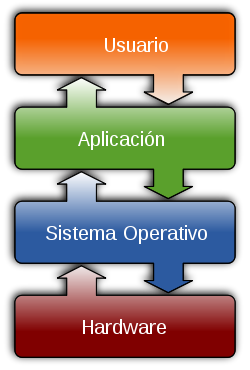
\includegraphics[width=0.25\textwidth]{imagenes/capas.png}}
\caption{Diagrama de capas.}
\end{figure}

El diseño del sistema esta bastante influenciado por \emph{Understanding The Linux Kernel, 3rd Edition} y \emph{Operating Systems Design and Implementation 2nd Edition, Tanenbaum}. Propone un sistema de segmentación flat, paginación y multi task.

\newpage
\section{Organizaci\'on del C\'odigo Fuente}
% \addcontentsline{toc}{section}{Organizaci\'on del C\'odigo Fuente}
A continuacion se presenta la jerarquia del codigo fuente.
\\
\\
\begin{figure}[H]
\centering
\subfloat{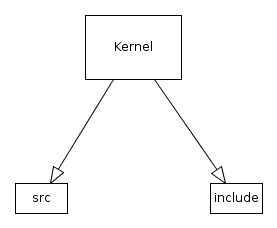
\includegraphics[width=0.5\textwidth]{imagenes/goblal.png}}
\caption{Diagrama de jerarquia de archivos.}
\end{figure}

\begin{figure}[H]
\centering
\subfloat{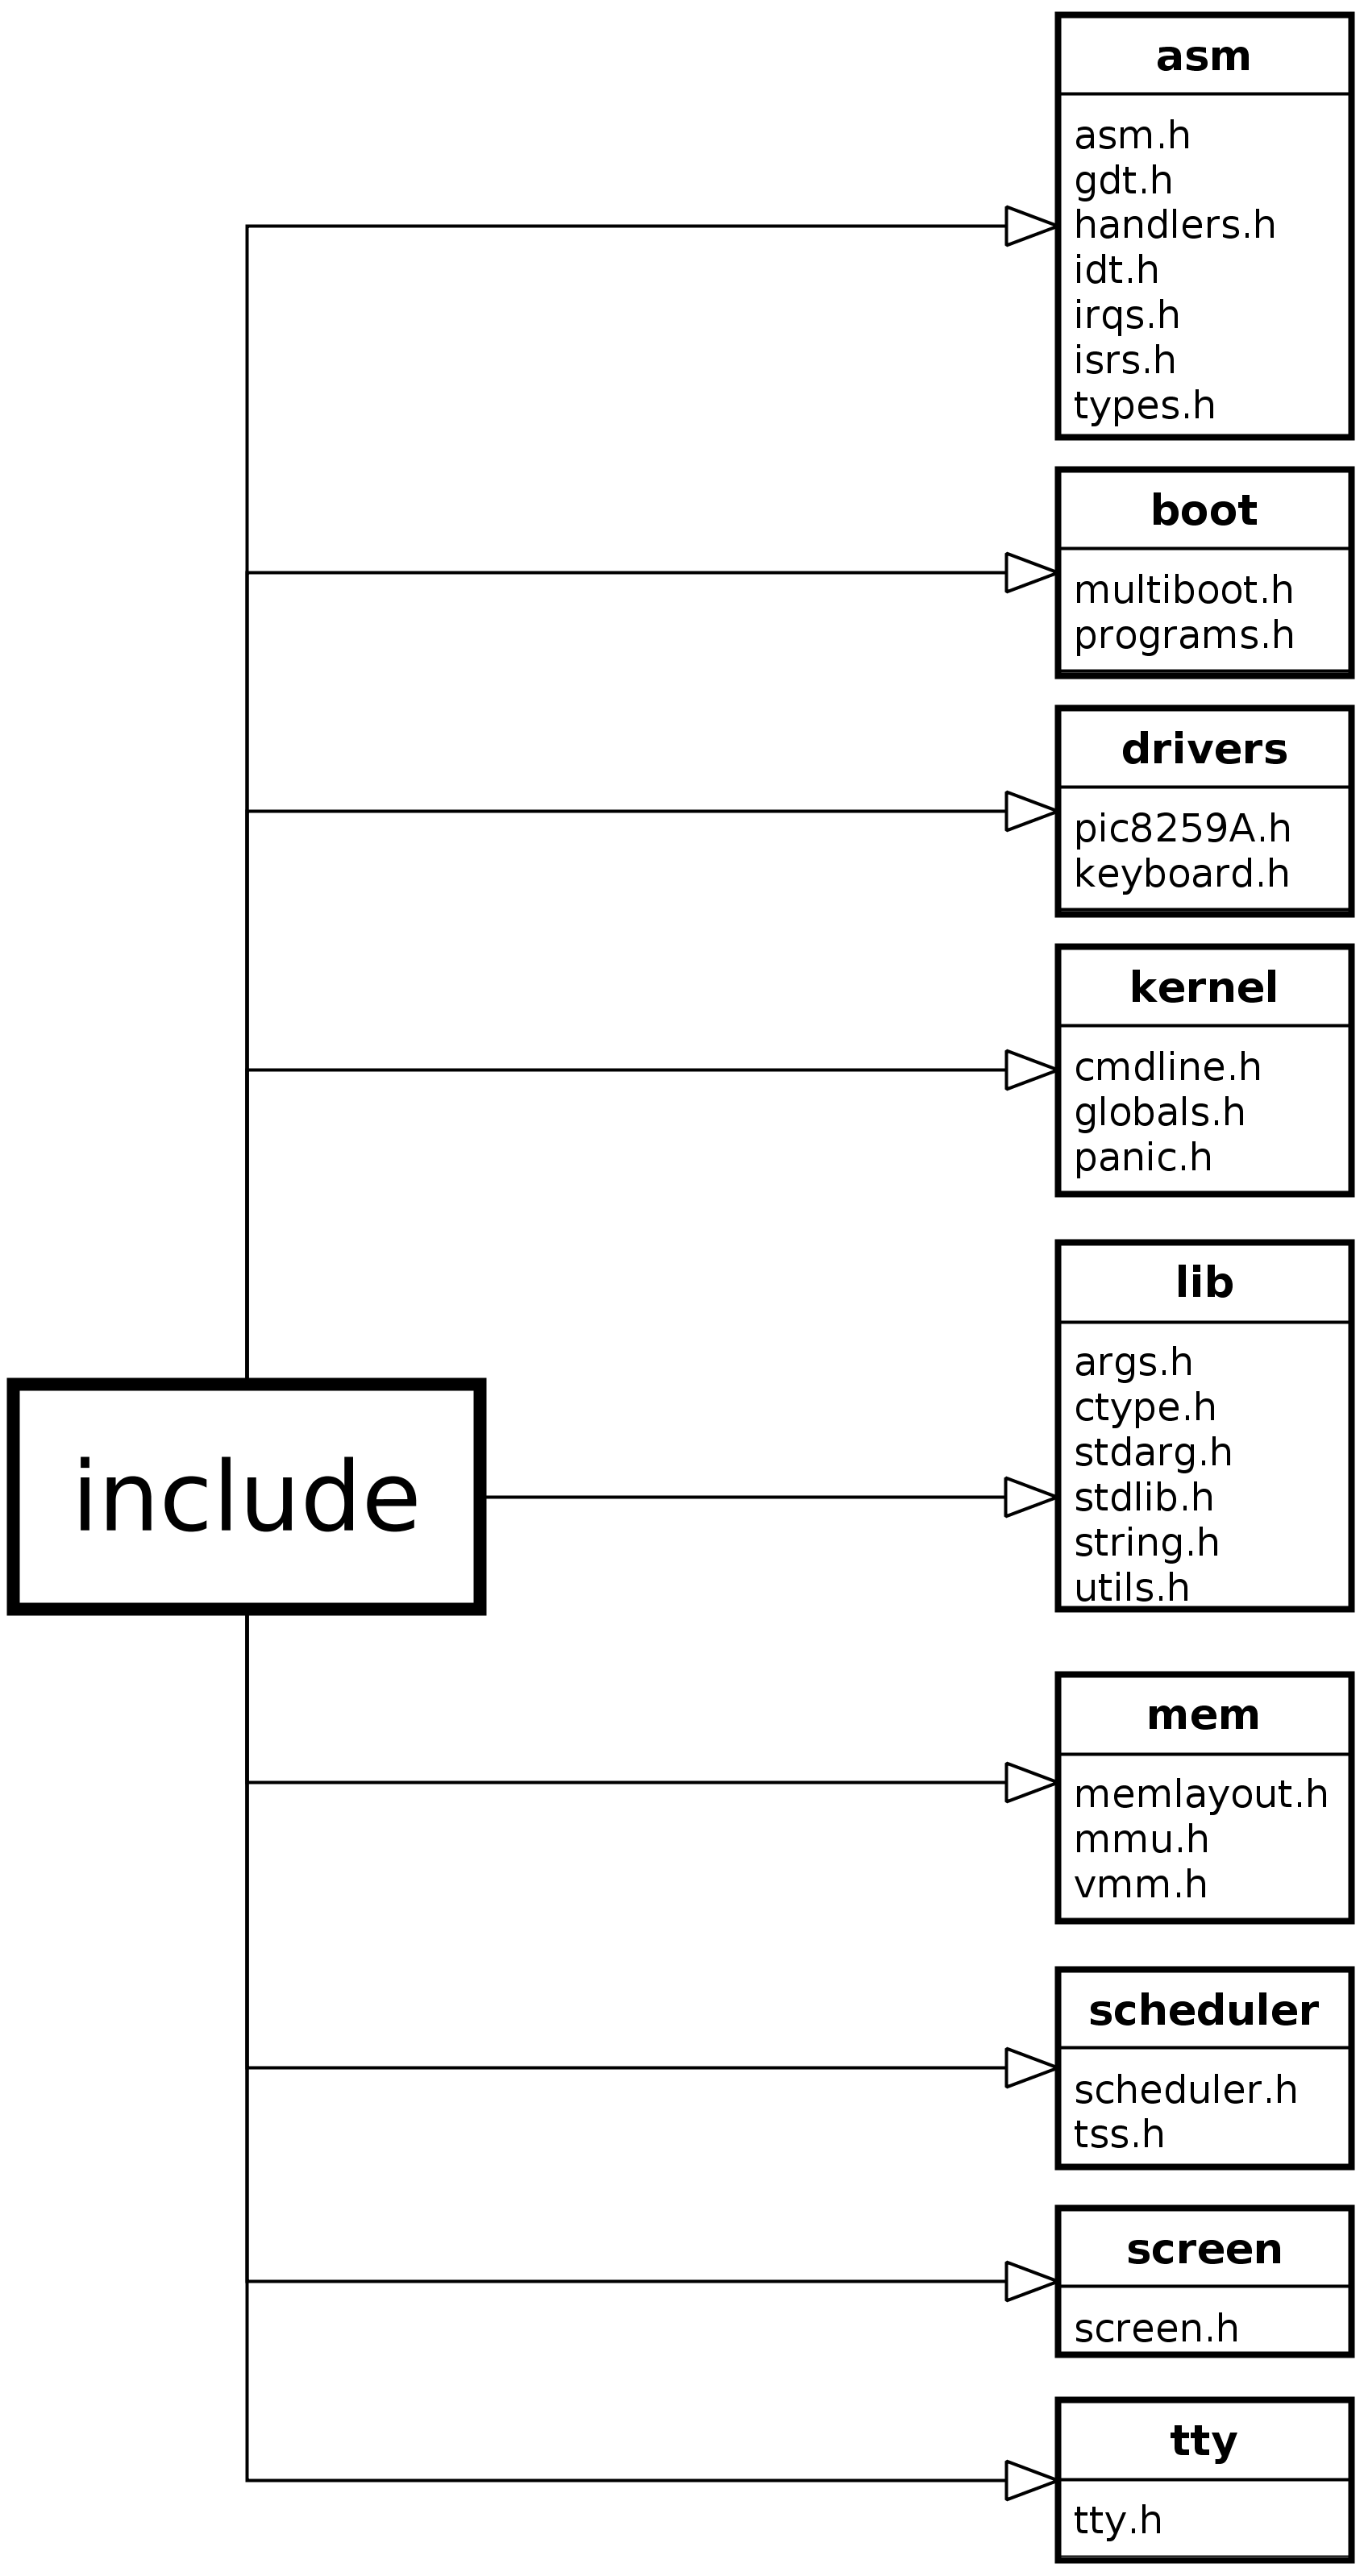
\includegraphics[width=0.5\textwidth]{imagenes/diagrama_de_archivos_include.png}}
\caption{Diagrama de jerarquia de archivos (cont).}
\end{figure}

\begin{figure}[H]
\centering
\subfloat{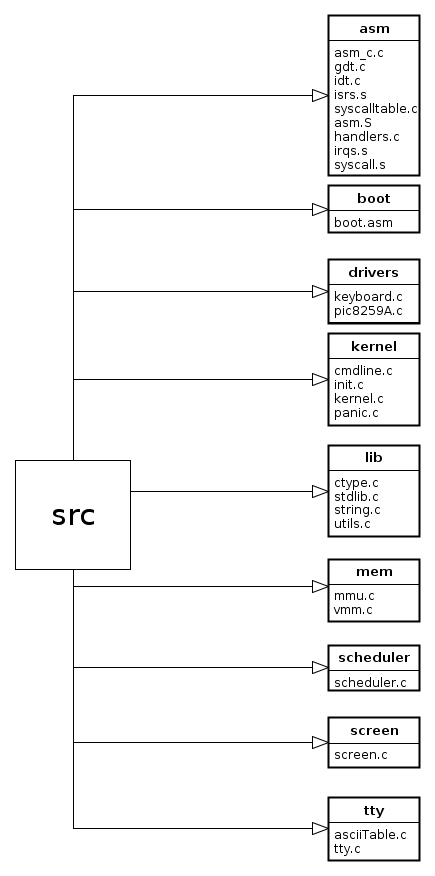
\includegraphics[width=0.5\textwidth]{imagenes/diagrama_de_archivos_src.png}}
\caption{Diagrama de jerarquia de archivos (cont).}
\end{figure}

\newpage
\section{Bootloader}
En cuanto al Bootloader, se barajaron varias opciones que se mencionan a continuación.

\subsection{GRUB}
Este bootloader cumple con la especificación multiboot. Cualquier bootloader que lo haga es capaz de bootear un archivo que cumpla con las siguientes propiedades:

Esté en formato ELF
Defina 3 enteros de 32 bits (en los primeros 8KB del archivo y alineados a 4 Bytes) con los siguientes datos (y en el siguiente orden):
0x1BADB002: Un número "mágico" para identificar esta estructura de datos.
flags: Un conjunto de bits que le indican a GRUB qué cosas hacer (además de cargarnos en memoria)
checksum: Una suma de comprobación para verificar que realmente se trata de la estructura adecuada. checksum = -(flags + 0x1BADB002)
Si no está en formato ELF, se lo puede indicar en los flags y luego indicarle a mano (agregando campos a la estructura) dónde cargar el código y demás.

\begin{itemize}
\item Ventajas
\\
Relativamente sencillo de aprender.
Puede bootear de practicamente cualquier medio.
Reconoce montones de sistemas de archivos: FAT, ext2, ext3, reiserfs, xfs, iso9660, etc.
Obtiene el mapa de memoria del BIOS y nos los pasa a nosotros.
Puede bootear archivos ELFs.

\item Desventajas
\\
Si bien sencillo, también requiere un poco de "setup" extra.
Muy pesado, demasiada funcionalidad para lo que podríamos necesitar.

\end{itemize}


\subsection{Lector de Sectores del Disco}
\begin{itemize}
\item Ventajas
\\
Sencillo de entender.
Sencillo de empezar a utilizar.
Extremadamente liviano.
La sensación de "lo hizimos nosotros" :P
Se pueden elegir los distintos drives cambiando el registro dl. La especificacion de como hacerlo esta en 

\item Desventajas
\\
No respeta ningún filesystem.
No provee información acerca del mapa de memoria.
No pasa argumentos al kernel.
No es flexible como GRUB.


\end{itemize}

\subsection{FAT32 Bootloader}

\begin{itemize}
\item Ventajas
\\
Sencillo.
Pequeño.
Reconoce al menos un filesystem.

\item Desventajas 
\\
Reconoce sólo un filesystem.
Requiere modificaciones al código fuente para cumplir nuestras espectativas.
No provee información acerca del mapa de memoria.
No pasa argumentos al kernel.
No es flexible como GRUB.
\end{itemize}



\newpage
\section{MMU: Memory Management Unit}

\subsection{Introducción}
En cualquier kernel el manejo de memoria es una parte fundamental. Nuestro kernel no es la excepción. El kernel cuenta con dos niveles de administración
de memoria. De estos dos niveles, la \textit{Unidad de Administración de Memoria}, o \textit{MMU} por sus siglas en inglés (Memory Management Unit) se encarga de administrar la memoria física. 
Es decir, de manejar correctamente y lo mejor posible las páginas y todo lo que concierne al respecto. \\
El modelo de memoria elegido para nuestro kernel hace uso de paginación, aunque no asi de la unidad de Segmentación (sólo lo mínimo necesario para ser funcional). La mmu se encarga entonces 
de administrar las páginas físicas. La forma de administración es relativamente sencilla para el nivel de complejidad del kernel. Los marcos de páginas libres se mantienen en una pila, 
pudiendo extraer del mismo y asociarlos a direcciones virtuales. También se permite liberarlos devolviéndolos a la pila. A continuación se explica más detalladamente cómo se administra la memoria 
y las funciones y mecanismos para ello.

\subsection{Estructuras de la MMU}
La memoria física se divide en unidades de tamaño 4kb llamadas frames o marcos de página. Cada vez que la mmu otorga un sector de memoria a una tarea u otro módulo del kernel que lo requiera, lo 
hace en estas unidades básicas. La tarea principal de la MMU será entonces mantener de alguna forma coherente, la cantidad de frames que aún quedan libres, cuales son, y cuales están siendo ocupados.

\begin{figure}[H]
\centering
\subfloat{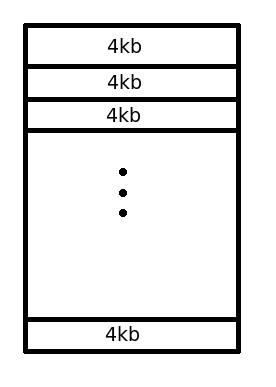
\includegraphics[width=0.4\textwidth]{imagenes/mmu_page_frames.png}}
\caption{Memoria física dividida en sectores contiguos de tamaño 4kb}
\end{figure}

Cada frame de la memoria física se representa con la siguiente estructura

\begin{verbatimtab}
typedef struct page_frame
{
   struct page_frame* next; //proximo frame de la lista de frames libres
   struct page_frame* prev; //frame anterior de la lista de frames libres
   uint32_t ref_count;  //cantidad de referencias externas
} page_frame_t;
\end{verbatimtab}

La mmu mantiene un array llamado \textit{mem\_page\_frames} de estructuras \textit{page\_frame\_t}, una por cada frame físico. A su vez existe una pila de frames libres apuntada por 
\textit{free\_page\_frame\_stack}. Los punteros \textit{next} y \textit{prev} sirven entonces para formar una lista doblemente enlazada entre los frames que esten libres. Un frame esta libre 
si y sólo si su cantidad de referencias es nula. Es decir, no existe ninguna virtual address de ninguna tarea ni proceso que haga referencia al frame. De esta forma se obtiene una estructura 
como la que se muestra a continuación:

\begin{figure}[H]
\centering
\subfloat{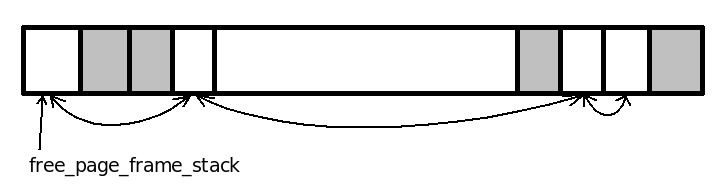
\includegraphics[width=0.8\textwidth]{imagenes/mmu_page_frames_array.png}}
\caption{Memoria física dividida en sectores contiguos de tamaño 4kb}
\end{figure}

\subsection{Inicialización de la MMU}
Para poder construir la estructura anteriormente descripta, es necesario que el kernel conozca la cantidad de memoria con la que cuenta. La mmu cuenta con una función que se encarga de inicializar 
todo lo necesario, incluyendo un conteo de la cantidad de memoria total. Este trabajo es llevado a cabo por la función \textit{mmu\_init}. El prototipo de la función es 

\begin{verbatimtab}
 /**
 * Inicializa la Memory Management Unit. Para ello utilizando la informacion provista 
 * por GRUB inicializa las estructuras de control de memoria y se encarga de llamar 
 * a las funciones necesarias para instalar la GDT definitiva y pasar a paginacion
 *
 * @param mdb Puntero a estructura multiboot_info_t provista por GRUB al inicio del kernel
 * @see mmu_install_gdt
 * @see mmu_init_paging
 * @see mmu_build_kernel_heap
 */
void mmu_init(multiboot_info_t* mbd);
\end{verbatimtab}

La estructura \textit{multiboot\_info\_t} es una estructura provista por GRUB al momento de booteo. Esta estructura provee, entre otros datos, un mapa de la memoria física, describiendo 
no sólo la cantidad de memoria disponible, sino también qué sectores están reservados por otros dispositivos como el BIOS y cuales están libres para uso del SO. Utilizando esto, la mmu 
inicializa el array de frames, marcando como ocupados aquellos que corresponden a sectores reservados. Un esquema simplificado de los pasos que realiza \textit{mmu\_init} sería

\begin{verbatimtab}
 mmu_init
      Contar la memoria disponible
      Correr el puntero __kernel_end tanto como ocupe mem_page_frames

      Para cada frame
	  Si la direccion del frame corresponde a un sector reservado
	  o a una direccion del kernel, marcarlo como ocupado
	  Si no, como libre.

      Inicializar paginacion

      Instalar GDT definitiva
\end{verbatimtab}

\subsection{Paginación y la MMU}
Como ya dijimos, nuestro kernel utiliza el modelo de paginacón. El mapeo realizado por el kernel es bastante sencillo. Las direcciones del kernel comienzan a partir de 0x80000000, mientras que 
el espacio de usuario esta reservado entre los 0 y 2 primeros GB. Para que el kernel utilice estas direcciones, es linkeado por un linker script especial. Sin embargo, el bootloader carga 
el kernel en las primeras direcciones. Para poder ejecutar el código sin problemas, se instala una GDT provisoria, cuyos segmentos son especialmente definidos para que cuando la unidad de segmentación 
traduce las direcciones, la dirección resultante sea \textit{d} + 0x80000000. De esta forma el código puede ejecutar sin problemas.\\
Dentro de \textit{mmu\_init} dijimos que se inicializan las estructuras de paginación. La PDT del kernel es apuntada por \textit{kernel\_pdt} (definida en mmu.c). La PDT se construye entonces 
mapeando el kernel desde los 2GB en adelante, utilizando páginas de 4mb para que las traducciones de la TLB se realice en forma más eficientemente ya que el procesador utiliza una TLB distinta.
Asi mismo, también se mapea el kernel a partir de la dirección 0x0 con un propósito: en el momento de transición entre activar paginación e instalar la GDT definitiva (recordando que teníamos una provisoria) 
todo siga funcionando. Cuando iniciamos paginación, comienza a actuar una unidad de traducción adicional de direcciones. Dado que sigue en acción la GDT provisoria, ahora las direcciones que antes 
eran físicas, pasan por la traducción de la PDT. Al haber mapeado el kernel a partir de 0x0 todo funciona correctamente. Finalmente instalamos una GDT definitiva utlizando segmentos de 4gb, por lo que 
las direcciones lineales ahora son traducidas por el mapeo desde los 2gb en adelante.

\subsection{Interfaz de la MMU}
Para que la MMU pueda ser utilizada, se define en mmu.h su interfaz pública. Las funciones que expone son las siguientes

\subsubsection{mmu\_alloc}
\begin{verbatimtab}
uint8_t mmu_alloc(uint32_t *pdt, uint32_t *va, uint32_t *pa, uint8_t perm);
\end{verbatimtab}
Toma un frame fisico libre de 4kb y lo mapea dentro de la primera direccion virtual disponible para la 
PDT pasada como parametro con los permisos solicitados. Devuelve ademas la direccion fisica asociada.\\
Parámetros:
\begin{itemize}
 \item \textbf{pd} Puntero a la pdt sobre la cual se quiere realizar el mapeo.
 \item \textbf{va} Puntero donde se guarda la direccion virtual donde se realizo el mapeo
 \item \textbf{pa} Puntero donde se guarda la direccion fisica
 \item \textbf{perm} Permisos asignados a la pagina mapeada
\end{itemize}


\subsubsection{mmu\_alloc\_at\_VA}
\begin{verbatimtab}
 uint8_t mmu_alloc_at_VA( pde_t *pdt, uint32_t va, uint8_t perm, uint8_t force_dealloc );
\end{verbatimtab}
Obtiene un frame libre y lo intenta mapear en la direccion virtual pasada como parametro.\\
Parámetros:
\begin{itemize}
 \item \textbf{pdt} Puntero a la PDT sobre la cual se realiza el mapeo
 \item \textbf{va} Direccion virtual usada para mapear el frame libre
 \item \textbf{perm} Permisos asignados a la nueva pagina mapeada
 \item \textbf{force\_dealloc} Si en la va pasada como parametro ya habia un mapeo previo, entonces lo deshace si force\_dealloc==1
\end{itemize}
Devuelve E\_MMU\_SUCCESS si se realizo el mapeo correctamente, E\_MMU\_INVALID\_VA si ya habia un mapeo y force\_dealloc==0 o E\_MMU\_NO\_MEMORY si no se pudo realizar.

\subsubsection{mmu\_map\_pa2va}
\begin{verbatimtab}
 uint8_t mmu_map_pa2va(pde_t *pdt, uint32_t pa, uint32_t va, uint8_t perm, uint8_t force_dealloc );
\end{verbatimtab}
Intenta asociar la va con la pa pasada como parametro para la pdt solicitada.\\
Parámetros:
\begin{itemize}
 \item \textbf{pdt} Puntero a la PDT sobre la cual se realiza el mapeo
 \item \textbf{va} Direccion fisica usada para realizar el mapeo
 \item \textbf{va} Direccion virtual usada para mapear la direccion fisica
 \item \textbf{perm} Permisos asignados a la nueva pagina mapeada
 \item \textbf{force\_dealloc} Si en la va pasada como parametro ya habia un mapeo previo, entonces lo deshace si force\_dealloc==1
\end{itemize}
Devuelve E\_MMU\_SUCCESS si se realizo el mapeo correctamente, E\_MMU\_INVALID\_VA si ya habia un mapeo y force\_dealloc==0 o E\_MMU\_NO\_MEMORY si no se pudo realizar

\subsubsection{mmu\_free}
\begin{verbatimtab}
 uint8_t mmu_free( pde_t *pdt, uint32_t va );
\end{verbatimtab}
Dada una PDT, deshace el mapeo de la va, obtiene el frame correspondiente, decrementa su cantidad de 
referencias (si son 0 lo apila como libre) y realiza invlpg para limpiar la TLB. \\
Parámetros:
\begin{itemize}
  \item \textbf{pdt} Puntero a una PDT.
  \item \textbf{va}  Direccion virtual a liberar. Debe ser multiplo de PAGE\_SIZE
\end{itemize}
Devuelve E\_MMU\_SUCCESS si la operacion se realizo con exito, o E\_MMU\_INVALID\_VA si la va no pudo ser desmapeada.

\subsubsection{mmu\_get\_free\_frame\_count}
Devuelve la cantidad de frames libres en memoria fisica
\begin{verbatimtab}
 mmu_get_free_frame_count(); 
\end{verbatimtab}

\subsubsection{mmu\_install\_task\_pdt}
\begin{verbatimtab}
 uint8_t mmu_install_task_pdt(uint32_t *va, uint32_t *pa);
\end{verbatimtab}
Instala una nueva PDT para ser usada por una nueva tarea.\\
Parámetros:
\begin{itemize}
 \item \textbf{va} Es un puntero a un uint32\_t que se va a utilizar para guardar la va utilizada para mapear la nueva pdt dentro del contexto del kernel.
 \item \textbf{pa} Es un puntero a un uint32\_t que se va a utililar para guardar la pa utilizada para guardar la nueva pdt.
\end{itemize}
Devuelve E\_MMU\_SUCCESS si se realizó con exito la instalación, o E\_MMU\_NO\_MEMORY si no hubo memoria disponible para realizar la operación.

\subsubsection{mmu\_kalloc}
\begin{verbatimtab}
 uint8_t mmu_kalloc( uint32_t *va );
\end{verbatimtab}
Toma un frame fisico libre de 4kb y devuelve su dirección virtual en el contexto del kernel.\\
Parámetros:
\begin{itemize}
  \item \textbf{va}  Puntero donde se guarda la dirección virtual.
\end{itemize}
Devuelve E\_MMU\_SUCCESS si se pudo realizar el alloc correctamente, o E\_MMU\_NO\_MEMORY en caso de error.


\subsection{Funciones internas de la MMU}
A continuación enumeramos las funciones definidas en mmu.c que no son parte de la interfaz pública

\subsubsection{mmu\_init\_paging}
\begin{verbatimtab}
static void mmu_init_paging(uint32_t *kpdt);
\end{verbatimtab}
Inicializa la PDT del kernel, mapeando la memoria fisica en forma lineal a partir 
de KERNEL\_VIRTUAL\_START utilizando paginas de KERNEL\_PAGE\_SIZE (4mb). \\
Parámetros:
\begin{itemize}
 \item \textbf{kpdt} Puntero a la page directory table del kernel
\end{itemize}

\subsubsection{mmu\_install\_gdt}
\begin{verbatimtab}
static void mmu_install_gdt();
\end{verbatimtab}
Instala la GDT definitiva, quitando la dummy gdt utilizada durante el proceso de booteo.

\subsubsection{mmu\_push\_free\_frame}
\begin{verbatimtab}
static void mmu_push_free_frame(page_frame_t* page_frame);
\end{verbatimtab}
Toma un puntero a un frame y lo almacena en la pila de frames libres. Solo se debe hacer push de frames con cantidad de referencias igual a 0. \\
Parámetros:
\begin{itemize}
 \item \textbf{page\_frame} Puntero al page\_frame\_t a liberar
\end{itemize}

\subsubsection{mmu\_pop\_free\_frame}
\begin{verbatimtab}
static page_frame_t* mmu_pop_free_frame();
\end{verbatimtab}
Saca un frame del stack de frames libres y devuelve un puntero a este. \\
Devuelve un puntero del tipo\textit{ page\_frame\_t*}. Si no hay frames libres, devuelve NULL.

\subsubsection{mmu\_page\_frame\_2\_PA}
\begin{verbatimtab}
static uint32_t mmu_page_frame_2_PA(page_frame_t* page_frame);
\end{verbatimtab}
Devuelve la direccion fisica del frame pasado como parametro. Para ello se fija en el puntero al frame, y lo compara con el puntero 
al principio de la lista para conocer su posicion y luego multiplicar convenientemente para conocer la direccion fisica del mismo.\\
Parámetros:
 \begin{itemize}
  \item \textbf{page\_frame} Puntero al page\_frame cuya physical address se quiere conocer
 \end{itemize}

\subsubsection{mmu\_PA\_2\_page\_frame}
\begin{verbatimtab}
static page_frame_t* mmu_PA_2_page_frame(uint32_t physical_address);
\end{verbatimtab}
Toma una direccion fisica y devuelve un puntero page\_frame\_t al frame correspondiente en el array 
mem\_page\_frames. No quita el frame de la lista de libres.\\
Parámetros:
\begin{itemize}
 \item \textbf{physical\_address} Direccion fisica del frame. Debe ser multiplo de PAGE\_SIZE.
\end{itemize}
Devuelve un puntero page\_frame\_t* al frame asociado, o NULL si la direccion fisica es inválida.

\subsubsection{ mmu\_get\_page\_frame}
\begin{verbatimtab}
static page_frame_t* mmu_get_page_frame(uint32_t physical_address);
\end{verbatimtab}
Dada una direccion fisica, devuelve el frame asociado a esta, pero lo quita de la lista de libres (si es que lo estaba) incrementando la cantidad de referencias.\\
Parámetros:
\begin{itemize}
 \item \textbf{physical\_address} Direccion fisica del frame. Debe ser multiplo de PAGE\_SIZE.
\end{itemize}
Devuelve un puntero page\_frame\_t* al frame asociado, o NULL si la direccion fisica es inválida.


\subsubsection{mmu\_free\_page\_frame}
\begin{itemize}
 \item \textbf{frame} Puntero al frame a liberar
\end{itemize}
Decrementa las referencias del frame pasado como parametro. Si llegan a ser nulas, se agrega a la pila de libres.


\subsubsection{mmu\_alloc\_page}
\begin{verbatimtab}
 static uint8_t mmu_alloc_page(pde_t *pdt, page_frame_t *page_frame, uint32_t va, uint8_t perm, uint8_t force_dealloc);
\end{verbatimtab}
Asocia la direccion virtual va con el frame apuntado por page\_frame para la PDT pasada como parametro, utilizando los permisos perm. 
Si la va ya estaba siendo utilizada para otro mapeo, force\_dealloc indica si se deshace el mapeo anterior o no.\\
Parámetros:
 \begin{itemize}
  \item \textbf{pdt} Puntero a la PDT sobre la cual se va a realizar el mapeo.
  \item \textbf{page\_frame} Puntero a un marco de pagina.
  \item \textbf{va} Virtual address a utilizar para el mapeo.
  \item \textbf{perm} Permisos con los que se va a mapear la pagina.
  \item \textbf{force\_dealloc} Si vale 1, fuerza el desmapeo de cualquier mapeo anterior.
 \end{itemize}
Devuelve E\_MMU\_SUCCESS si todo salio correctamente. E\_MMU\_INVALID\_VA si la va ya estaba mapeada y force\_dealloc==0. E\_MMU\_NO\_MEMORY si no hubo memoria.

\subsubsection{mmu\_dirwalk}
\begin{verbatimtab}
 static uint8_t mmu_dirwalk(pde_t *pdt, uint32_t va, pte_t **pte, uint8_t create_page_table, uint8_t ptable_domain);
\end{verbatimtab}
Recorre las tablas y hace apuntar pte a la page table entry que corresponde de acuerdo a la va pasada como parametro y la PDT. \\
Parámetros:
\begin{itemize}
  \item \textbf{pdt} Puntero a la PDT sobre la cual se va a realizar el mapeo.
  \item \textbf{va} Virtual address a utilizar para el mapeo.
  \item \textbf{pte} Puntero doble a una pte\_t. Dentro de pte se guarda la pte correspondiente a la va para la PDT.
  \item \textbf{create\_page\_table} Si la va no tiene una page table creada, create\_page\_table==1 hace que se cree dicha tabla, de lo contrario no se crea y mmu\_dirwalk devuelve error
\end{itemize}
Devuelve E\_MMU\_SUCCESS si todo salio correctamente. E\_MMU\_PTABLE\_NOT\_PRESENT si la tabla de paginas para la va no existe y create\_page\_table==0. 
 E\_MMU\_NO\_MEMORY si no hubo memoria suficiente para realizar la operacion. 

\subsubsection{mmu\_get\_pte}
\begin{verbatimtab}
 static pte_t* mmu_get_pte(pde_t *ptd, uint32_t va);
\end{verbatimtab}
Devuelve un puntero a la la pte asociada a la va pasada como parámetro.\\
\begin{itemize}
  \item \textbf{pdt} Puntero a la PDT sobre la cual se va a realizar el mapeo.
  \item \textbf{va} Virtual address a utilizar para el mapeo.
\end{itemize}
Devuelve un puntero a la pte asociada o NULL si no existe la page table.

\newpage


\section{VMM Kernel Heap}
\subsection{Introducción}
Asi como existe la MMU que se encarga de administrar la memoria fsica, es decir, administrar los frames fsicos de 4kb, la unidad de memoria virtual esta encargada de administrar la memoria asignada 
de forma tal de poder otorgar punteros a sectores del tamao pedido. Bsicamente, nuestra vmm es una implementacin de malloc para uso del heap. No contamos con malloc para las tareas.

\subsection{Administracin del kernel heap}
La nica tarea que tiene soporte para uso de memoria dinnima en nuestro kernel es el mismo kernel. Para el manejo del heap se utiliza un mapeo especial dedicado al heap. La direccin donde se mapea 
el heap esta definida por KERNEL\_HEAP\_START (0xC0000000). Las funciones de la vmm se definen en vmm.h y vmm.c. La implementacin de kmalloc esta basada en la implementacin sugerida en 
\textit{The C language programming}, en la que el heap se administra en bloques de tamao variable. Cada bloque posee en su direccin ms baja la siguiente estructura:

\begin{verbatim}
union header{
    struct {
        //puntero al proximo bloque libre
        union header *ptr;
        //Tamao del bloque
        uint32_t size;       
    } s;
    
    //Solamente para alinear bien el header (el tipo align_t segun K&R puede variar segun la maquina)
    align_t x;
};
\end{verbatim}
Cada bloque de memoria del heap comienza con esta estructura, que es usada por kmalloc y kfree para saber donde est el prximo bloque de memoria 
libre, y que tamao tiene el bloque actual. De esta forma, la memoria fsica del heap queda estructurada como la siguiente figura:

\begin{figure}[H]
\centering
\subfloat{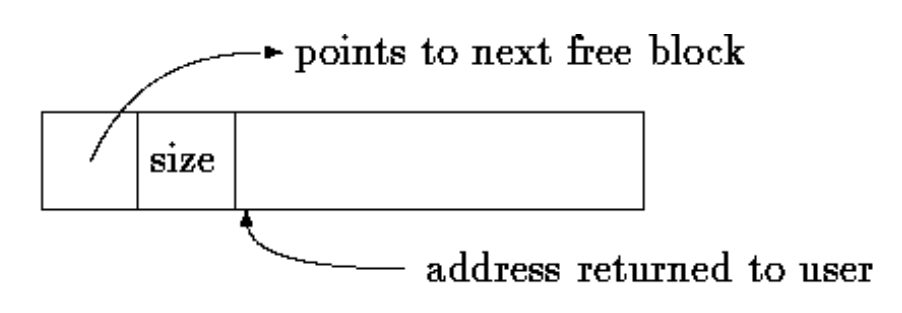
\includegraphics[width=0.4\textwidth]{imagenes/vmm_kmalloc_block.png}}
\caption{Un bloque de memoria del heap}
\end{figure}

\begin{figure}[H]
\centering
\subfloat{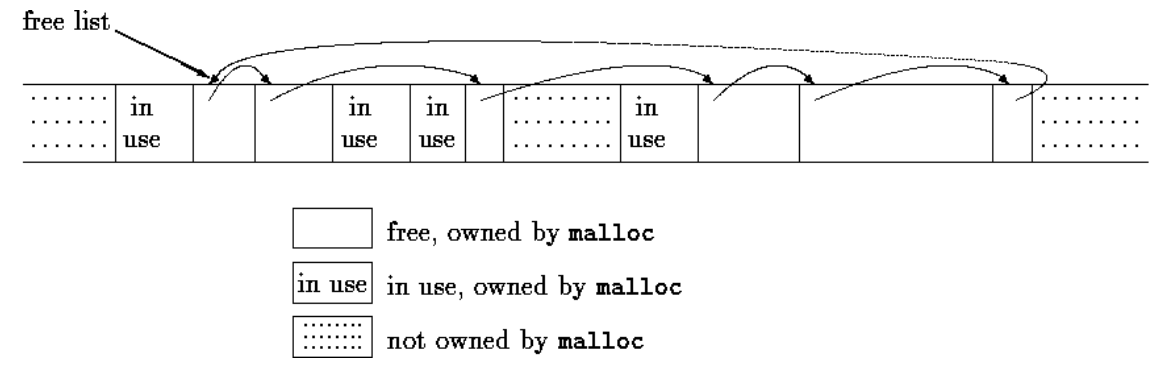
\includegraphics[width=0.4\textwidth]{imagenes/vmm_kmalloc_heap.png}}
\caption{Un bloque de memoria del heap}
\end{figure}

\subsubsection{ kmalloc }
La definicin de kmalloc es la siguiente

\begin{verbatim}
/**
 * Devuelve un puntero a block_size bytes listos para usar dentro del heap del kernel
 * No realiza verificacion de limites, por lo que escribir mas alla del tamao pedido puede ocasionar sobreescribir estructuras de control
 *
 * @param block_size Tamao del nuevo bloque pedido
 * @return ptr_t Puntero al bloque de memoria solicitado
 * @see kfree
 */
ptr_t kmalloc(uint32_t block_size);
\end{verbatim}

El algortmo usado por kmalloc es \textit{First fit}, es decir, cuando kmalloc busca un bloque de tamao block\_size, no busca el mejor para fragmentar menos la memoria, sino que usa el primero que encuentra de tamao mayor o igual. Si el bloque coincide con el tamao solicitado, entonces usa ese. Si en cambio encuentra primero un bloque de tamao mayor, divide el bloque en dos nuevos bloques: uno del tamao solicitado, y otro del tamao restante. Y devuelve el nuevo bloque creado. Si no encuentra bloques para alojar el tamao solicitado, pide al kernel ms espacio para el heap (no intenta reacomodar los bloques libres para generar uno de mayor tamao).

\subsubsection{ kfree }
Kfree esta definida como
\begin{verbatim}
/**
 * Libera un bloque de memoria solicitado con kmalloc.
 *
 * @param prt Puntero al bloque de memoria conseguido con kmalloc
 * @see kmalloc
 */
void kfree(ptr_t ptr);
\end{verbatim}

Kfree al igual que kmalloc libera la memoria siguiendo un algoritmo \textit{First fit}. Recorre el heap buscando una posicin para liberar el bloque. Si encuentra un bloque libre, entonces fusiona ambos bloques para generar uno de mayor tamao y asi reducir la fragmentacin.\\
Cabe aclarar que kfree nunca pide que el heap se achique, siempre se generan bloques ms grandes. Podra eventualmente detectar bloques excesivamente grandes 
y pedir al kernel que libere esas páginas.

\subsubsection{morecore}
La funcin \textit{morecore} es invocada por kmalloc cuando necesita ms espacio para el heap. La definicin es:
\begin{verbatim}
/**
 * Intenta agrandar el heap del kernel reservando mas espacio usand vmm_resize_heap.
 * 
 * @param size Tamao a agrandar
 * @return header_t* Devuelve un puntero al bloque de memoria conseguido, o NULL si no pudo agrandar el heap.
 * @see 
 */
static header_t* vmm_morecore(uint32_t size);
\end{verbatim}
La funcin de morecore es determinar cuntos bytes va a solicitar al kernel, para luego hacer la solicitud mediante la función \textit{vmm\_resize\_heap}

\subsubsection{vmm\_resize\_heap}
\begin{verbatim}
/**
 * Agranda el heap en nbytes bytes.
 *
 * @param nbytes Cantidad de bytes para agrandar el heap
 * @return uint8_t* Puntero al bloque de nbytes bytes.
 * @see vmm_morecore
 */
static uint8_t* vmm_resize_heap(uint32_t nbytes);
\end{verbatim}
Dentro de vmm\_resize\_heap se determina la cantidad entera de pginas de 4kb que son necesarias pedir a la mmu, y el pedido se realiza utilizando la funcin \textit{mmu\_alloc\_at\_VA}. Se especifica la VA del pedido para que el heap se agrande manteniendo la continuidad de las direcciones y asi poder pedirle a kmalloc bloques de ms de 4kb y que funcione correctamente.

\newpage
\section{Scheduler}

Para la realizaci\'on del Scheduler se implement\'o una pol\'itica de Round Robin. Cada tarea tiene un quantum variable que se gasta cada 1 timertick y al terminar éste se pasa a la ejecuci\'on de la siguiente tarea.
Se uso fuertemente en este la funcionalidad del mmu, por lo cual se serializo el trabajo.

Toda la funcionalidad del Scheduler se encuentra en tres archivos:
\begin{itemize}
\item	- scheduler.h
\item	- tss.h
\item	- scheduler.c
\end{itemize}

En la cual podemos encontrar la siguiente estructura que define a una tarea.

\begin{verbatim}
      typedef struct {
          char hay_tarea;						
          unsigned int quantum_fijo;			
          unsigned int quantum_actual;		
          char *pantalla;					
          void *va_tss;						
          void *pa_tss;						
      } tarea;
\end{verbatim}

Contamos con las siguientes variables globales:

\begin{verbatim}
      tarea tareas[10];
      char tarea_activa;	
      char tarea_en_pantalla;
      char contador_actualizar_pantalla;
      programs_t* programas[5];
\end{verbatim}


Y con las siguientes funciones:

\begin{itemize}
\item \begin{verbatim}void menu(); \end{verbatim}
\item \begin{verbatim}void scheduler();\end{verbatim}
\item \begin{verbatim}void matar_tarea(char numero_tarea);\end{verbatim}
\item \begin{verbatim}void mostrar_slot(char s);\end{verbatim}
\item \begin{verbatim}void iniciar_scheduler();\end{verbatim}
\item \begin{verbatim}void crear_tarea(programs_t programa, char numero_tarea);\end{verbatim}
\end{itemize}

\subsection{void menu()}
Es el procedimiento encargado mostrar el menu de texto (el cual explica la operatoria) por pantalla.

\subsection{void scheduler()}
Es el procedimiento encargado de pasar a la siguiente tarea, consultando las variables globales, elije la próxima tarea y hace un jmp a ella. Modificando las variables correspondientes para conservar la coherencia.

\subsection{void matar\_tarea(char numero\_tarea) }
Es el procedimiento encargado de desalojar la tarea \begin{it}numero\_tarea\end{it} del sistema. Libera toda la memoria que pidio al iniciarla y actualiza variables para conservar la coherencia.

\subsection{void mostrar\_slot(char s)}
Es el procedimiento encargado de mostrar en pantalla la tarea \begin{it}s\end{it} pasada como argumento. Pasando del buffer de pantalla de \begin{it}s\end{it} a la pantalla real, la informacion correspondiente.

\subsection{void iniciar\_scheduler()}
Es el procedimiento encargado de setear todas las variables iniciales para el buen funcionamiento del schduler. También lanza el menu.

\subsection{void crear\_tarea(programs\_t programa, char numero\_tarea)}
Es el procedimiento encargado de ingresar un programa al sistema, conviertiendolo en tarea. Se ejecuta en un entorno Kernel.
El siguiente pseudocodigo especifica su función.
\begin{verbatim}
void crear_tarea(programs programa, char numero_tarea){
    
    Deshabilitamos Interrupciones.
    Si existe tarea corriendo en slot numero_tarea la matamos.
    Creamos nuevo directorio tabla de pagina.
    Creamos tss para nueva tarea.
    Pedimos paginas para codigo y mapeamos en el DTP de la tarea a ingresar.
    Copiamos codigo a paginas pedidas.
    Pedimos pagina para pila y mapeamos en el DTP de la tarea a ingresar.
    Modificamos GDT para agregar el Descriptor correspondiente a esta tarea.
    Llenamos tss con los datos validos.
    Creamos buffer de video para nueva tarea.
    Mapeamos la 0xb8000 al DTP de la nueva tarea a su buffer.
    Modificamos las variables correspondientes al scheduler.
    Habilitamos interrupciones.
}
\end{verbatim}









\newpage
\section{Teclado y TTY (o Prompt)}
Fue necesario para poder interactuar con el sistema implementar un controlador de teclado simple y . El cual permitiera de forma básica aprovechar la interacción del usuario con el sistema. Para ello implementamos una serie de funciones (ubicadas en keyboard.c). Este driver funciona en conjunto con un módulo llamado tty ofreciendo varias funcionalidades.\\
Tales funcionalidades son registrar una función a una tecla de modo que cuando se pulse esa tecla en vez de ingresarse al prompt se dispare la suscitada función. También lograr que tener la cantidad necesarios de "prompts" como se necesite, y configurar que cuando se introduzcan letras a través de ese prompt sean dirigidos al "prompt" correspondiete.

Para todo esto se provee la siguiente interfaz:

\begin{verbatim}

En el driver de video (screen.c)
    //funcion que recibe un caracter o una serie de ellos y los imprime en la zona de prompt
    size_t kprint_tty(uint8_t * );
    //funcion que limpia el prompt
    void kprint_tty_clear();
    //funcion para borrar un caracter
    void kprint_tty_backspace();


tty_buffer_out_f  //tipo de funcion que recibe el buffer que se escribe en el prompt

//los prompt o tty se pueden crear dinamicamente e ir guardando en una lista.
//es por eso que se utilizo esta estructura para guardar toda la informacion 
//necesarias para administrar cada uno de los prompt.
struct tty_tty_node {
    
    tty_t tty;
    uint8_t buff[MAX_TTY+2];
    uint32_t buff_pos;
    bool expects_char;
    bool expects_string;
    bool enabled;
    tty_buffer_out_f buffer_out;
    void * next;
};

/*escribe un caracter en el prompt */
void tty_put_key(key);
/*el proximo caracter que se presione se enviara a travez del tty_buffer_out_f asociado
 * solo si no se pidio */
bool tty_get_key(tty_t* tty);
/*la proxima linea que se ingrese se enviara a travez del tty_buffer_out_f asociado
 * solo si no se pidio */
bool tty_get_string(tty_t* tty);
/* inicializa el tty con 1 TTYs al comienzo */
int tty_init(tty_t* tty, tty_buffer_out_f out_f);
/* agrega un tty con un buffer asociado, tty es de salida, devuelve el tty asociado a esta vista. */
int tty_tty_add(tty_t* tty, tty_buffer_out_f out_f);
/* cambia al tty designado */
int tty_tty_change(tty_t* tty);
\end{verbatim}

Por lo que la idea es inicializar las tty con tty\_init, agregar todas las tty que se necesiten con tty\_add , e ir cambiando entre ellas con tty\_change. Se decidio implementar que siempre se recibe un puntero a tty\_t, lo cual funciona muy parecido a libreria pthread, de modo que es tanto entrada como salida segun como se necesite, cuando se crea se deja alli el valor, y para las demas acciones es de entrada. Por lo que el creador de cada tty debe administrar de alguna forma cada tty con los tty\_t.

Cada uno de estos tty permiten llamar a las funcion $tty\_get\_string$ y $tty\_get_char$ las cuales, en el momento que ocurra el evento deseado (tanto un enter como la entrada de un caracter), llamarán a la funcion previamente designada a este tty. Es importante notar que esta acción es asincronica, por lo que se deberia hacer polling (busy waiting) sobre algun variable de estado, o (más adelante) implementar que las tareas sean marcadas como ocupadas.

\newpage
\section{C\'omo usar el SO}
% \addcontentsline{toc}{section}{C\'omo usar el SO}
Para ir al menu se debe presionar la tecla Esc. Ahi mismo podra ingresar todo lo que el menu lo ofrece mediante las instruciones detalladas.
Con las teclas F1, F2,...,F10 podra moverse entre las tareas que tiene en ejecución.


\end{document}
